%----------------------------------------
% Write your notes here
%----------------------------------------

\section{Introduction}
\subsection{What is Classification?}

Classification is the problem of identifying to which of a set of categories (sub-populations) a new observation belongs, on the basis of a training set of data containing observations (or instances) whose category membership is known.

\subsubsection{Mathematical Definition}
%\\{\bfseries Mathematically-}
{\itshape Input:} As with regression, in a classification problem we start with measurements {$x_1$, $x_2$, . . , $x_n$} in an input space $X$.
\\{\itshape Output:} The discrete output space $Y$ is composed of K possible classes:\\
1. $Y$ = \{−1, +1\} or \{0, 1\} is called binary classification.\\
2. $Y$ = \{1, . . . , K\} is called multiclass classification.\\
Instead of a real-valued response, classification assigns x to a category. For pair ($x$, $y$), $y$ is the class of $x$.

\subsubsection{Defining a Classifier}
Classification uses a function $f$ (called a classifier) to map input $x$ to class $y$.\\

    $y$ = $f(x)$

\section{Naive Bayes Classifier}
Naive Bayes classifiers are a family of simple probabilistic classifiers based on applying Bayes theorem with strong (naive) independence assumptions between the features.
\subsection{Assumption} All naive Bayes classifiers assume that the value of a particular feature is independent of the value of any other feature, given the class variable.
\subsection{Bayes Theorem} A theorem describing how the conditional probability of each of a set of possible causes for a given observed outcome can be computed from knowledge of the probability of each cause and the conditional probability of the outcome of each cause.\\

Formula: 
\begin{equation}
P(\theta|{D}) = P(\theta ) \frac{P({D} |\theta)}{P({D})},
\end{equation}

\subsubsection{Disease Example}
Consider a hypothetical population of 10,000 people.

\begin{figure}[H]
  \begin{center}
    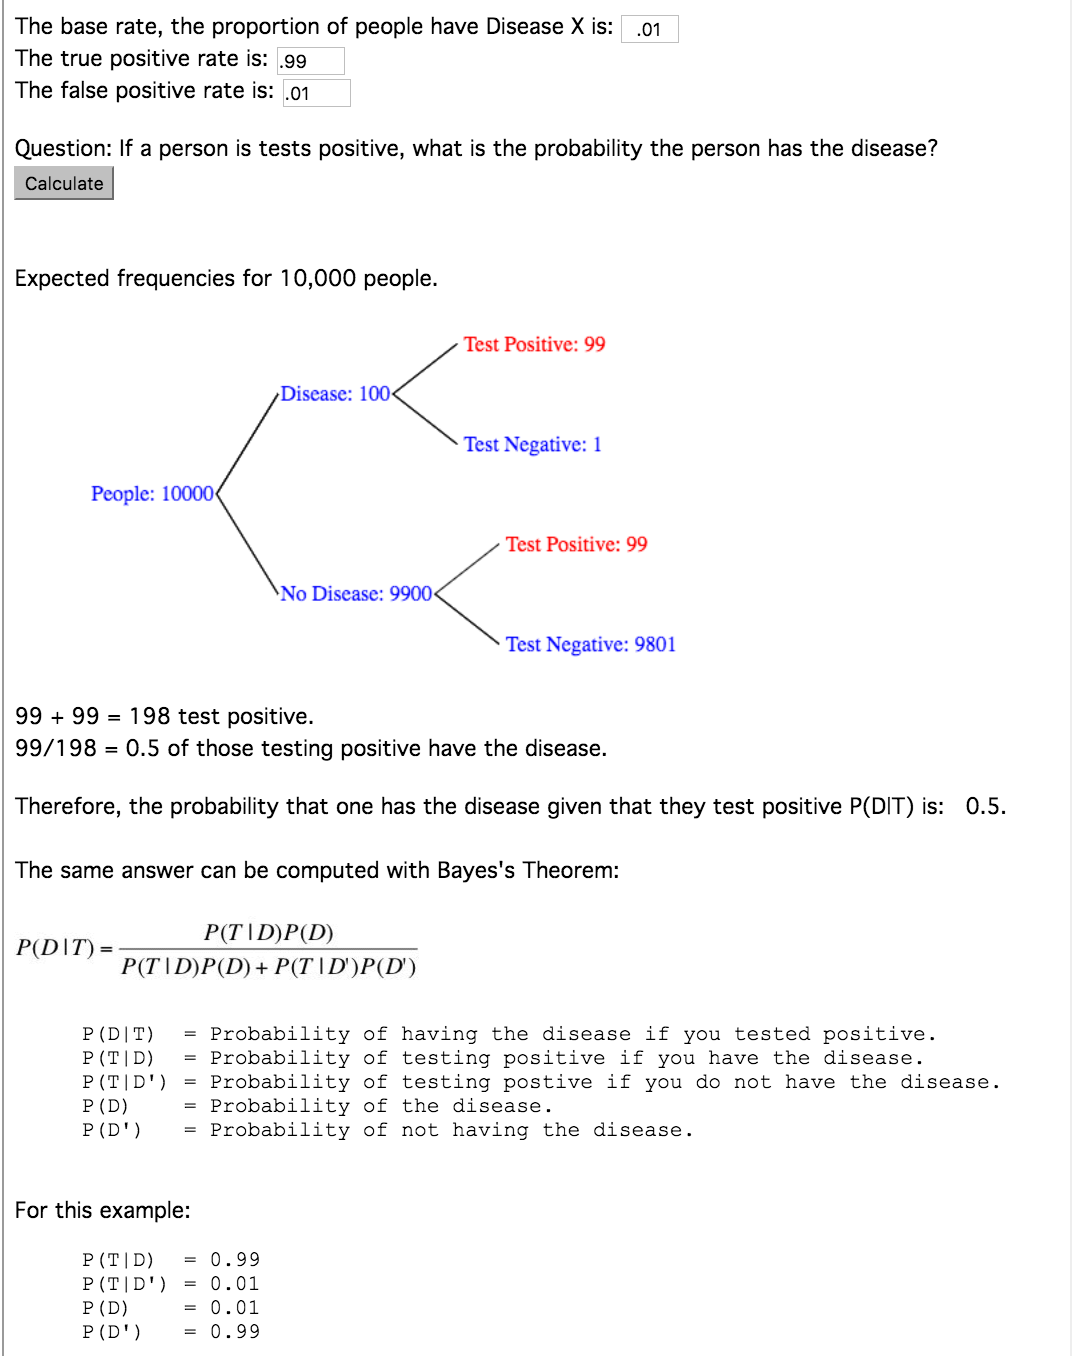
\includegraphics[width=0.5\textwidth]{disease_eg.png}
    \caption{
      Bayes Theorem Example (Source: http://onlinestatbook.com/2/probability/bayes\_demo.html)}
  \end{center}
\end{figure}

\subsection{Maximum Likelihood Estimate}
The probability of observing the data set in a class $C$, given parameters \(\theta\): (iid assumption)

\begin{figure}[H]
  \begin{center}
    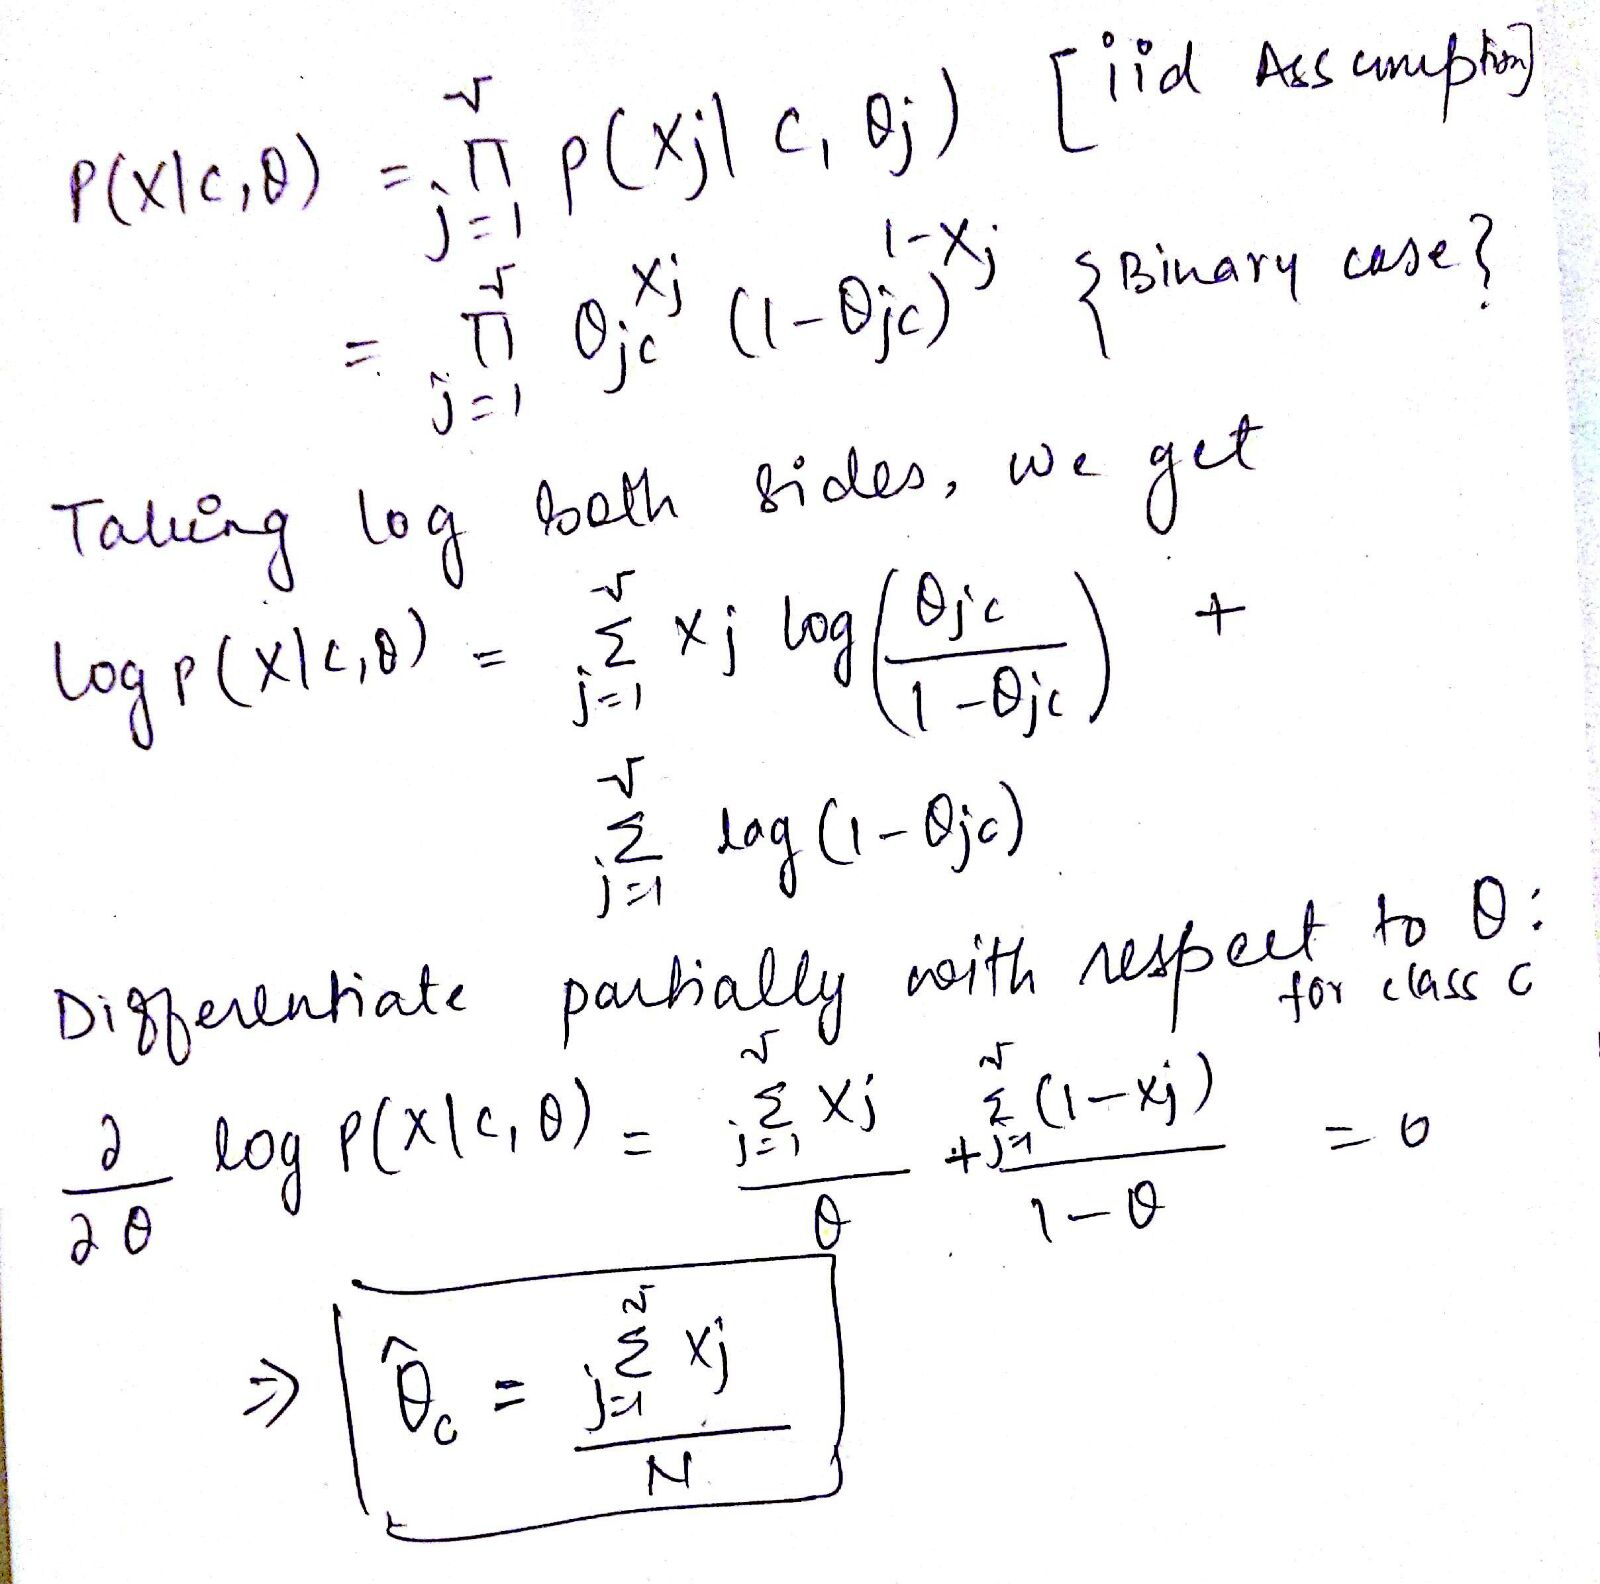
\includegraphics[width=0.5\textwidth]{mle.png}
    \caption{
      MLE for Naive Bayes}
  \end{center}
\end{figure}

\subsection{Advantages \& Disadvantages of Naive Bayes}
\subsubsection{Advantages}
\begin{itemize}
    \item Easy to implement
    \item Requires a small amount of training data to estimate the parameters
    \item Good results obtained in most of the cases
\end{itemize}

\subsubsection{Disadvantages}
\begin{itemize}
    \item Assumptions: class conditional independance, therefore loss of accuracy
    \item Practically, dependencies exist among variables
    \item Zero conditional probability problem
\end{itemize}

\subsection{Zero conditional probability problem explained}
\begin{itemize}
    \item If a given class and feature value never occur together in the training set then the frequency based probability estimate will be zero.
    \item This is problematic since it will wipe out all information in the other probabilities when they are multiplied.
    \item It is therefore often desirable to incorporate a small sample correction in all probability estimates such that no probability is ever set to be exactly zero.
    \item Laplace smoothing could be the one solution to eliminate this problem.
\end{itemize}

\section{Logistic Regression}

Logistic Regression removes the over-fitting by Naive Bayes for zero prior case. It doesn't assume the feature vectors to be uncorrelated.

\begin{figure}[H]
  \begin{center}
    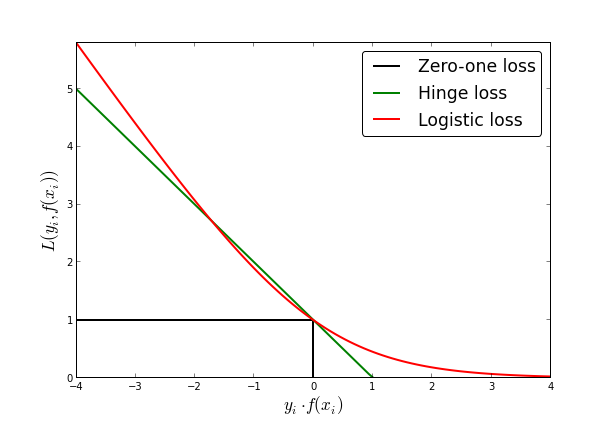
\includegraphics[width=0.5\textwidth]{loss_functions.png}
    \caption{
      Loss functions}
  \end{center}
\end{figure}

Binary Logistic Regression is a special type of regression where binary response variable is related to a set of explanatory variables, which can be discrete and/or continuous. The important point here to note is that in linear regression, the expected values of the response variable are modeled based on combination of values taken by the predictors. In logistic regression Probability or Odds of the response taking a particular value is modeled based on combination of values taken by the predictors. Like regression (and unlike log-linear models that we will see later), we make an explicit distinction between a response variable and one or more predictor (explanatory) variables.

\subsubsection{Log Odds Ratio}

\begin{figure}[H]
  \begin{center}
    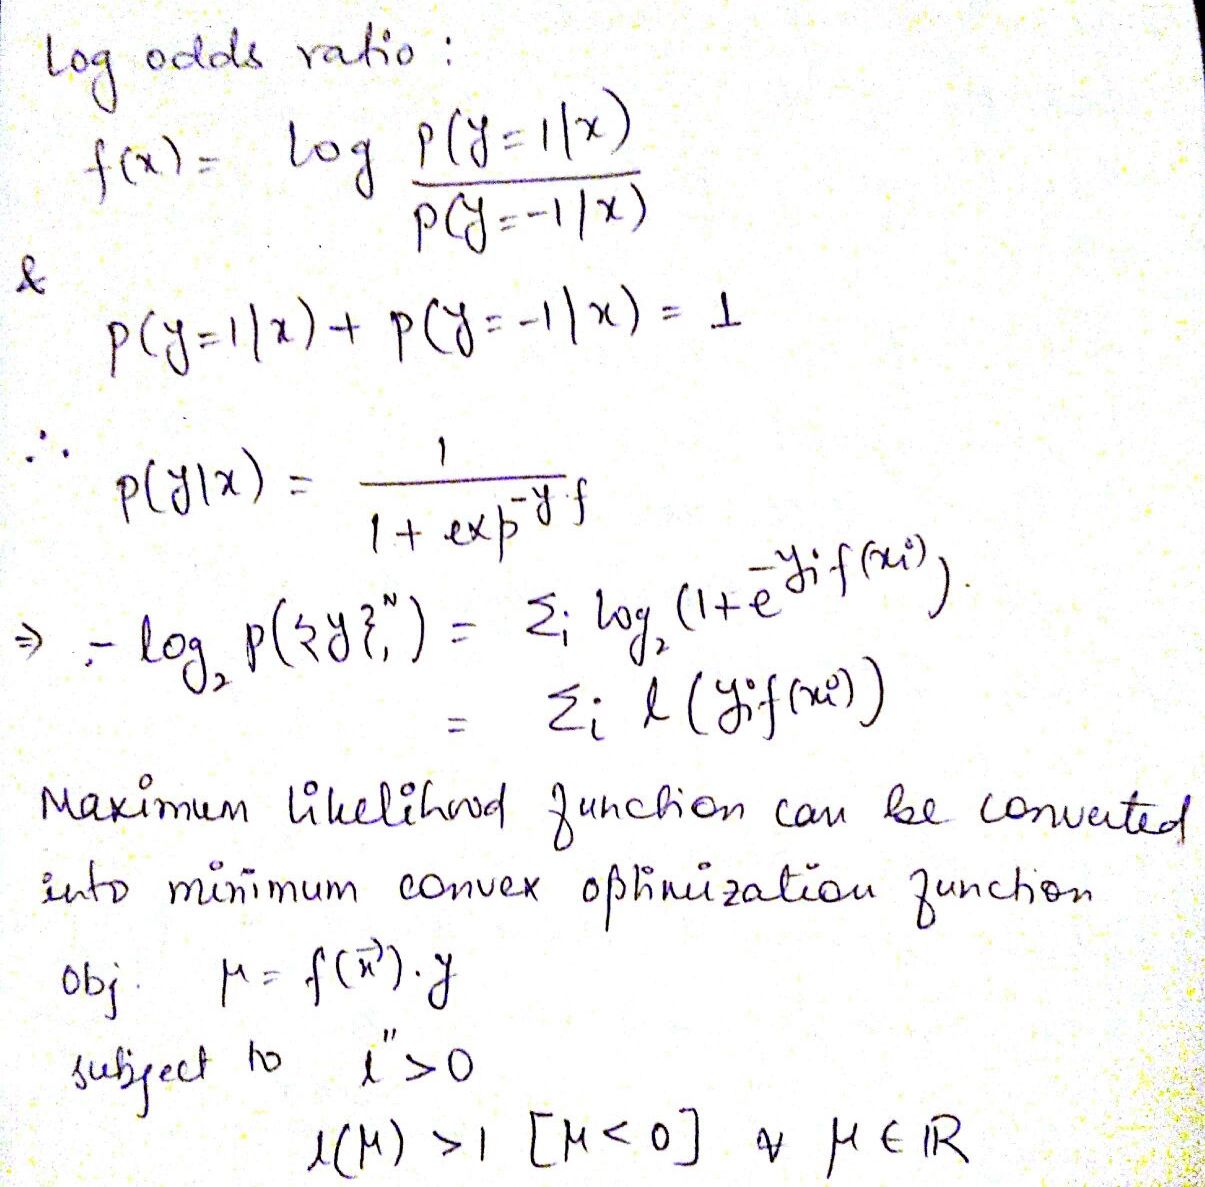
\includegraphics[width=0.5\textwidth]{log_odds.png}
    \caption{
      Log Odds Ratio: Logit Function}
  \end{center}
\end{figure}


Despite the probabilistic framework of logistic regression, all that logistic regression assumes is that there is one smooth linear decision boundary. It finds that linear decision boundary by making assumptions that the P(Y|X) of some form, like the inverse logit function applied to a weighted sum of our features. Then it finds the weights by a maximum likelihood approach. The decision boundary it creates is a linear decision boundary that can be of any direction.

\subsection{Advantages \& Disadvantages of Logistic Regression}
\subsubsection{Advantages}
\begin{itemize}
    \item Convenient probability scores for observations.
    \item Multi-collinearity is not really an issue and can be countered with L2 regularization to an extent.
\end{itemize}

\subsubsection{Disadvantages}
\begin{itemize}
    \item Doesn't perform well when feature space is too large.
    \item Doesn't handle large number of categorical features/variables well.
    \item Using MLE for parameter might not give closed form solution, therefore use iterative algorithms like Gradient descent (Boosting).
\end{itemize}

\subsection{Boosting}
While boosting is not algorithmically constrained, most boosting algorithms consist of iteratively learning weak classifiers with respect to a distribution and adding them to a final strong classifier. When they are added, they are typically weighted in some way that is usually related to the weak learners' accuracy. After a weak learner is added, the data are reweighted: examples that are misclassified gain weight and examples that are classified correctly lose weight. 











